\providecommand{\main}{../../../..}
\documentclass[\main/dresen_thesis.tex]{subfiles}
\begin{document}
  \label{sec:looselyPackedNS:layers:pnr}

  % \begin{table}[!htbp]
  %   \centering
  %   \caption{\label{tab:looselyPackedNP:nanoparticle:gisaxs}Parameters for the hard-sphere structure factor in Percus-Yervick approximation shown in \reffig{fig:looselyPackedNP:layer:gisaxs} for both SC-IOS-11 and SC-IOS-7. $R_\mathrm{HS}$ is the hard-sphere radius and $\eta$ the packing fraction of the structure factor.}
  %   \begin{tabular}{ c | l | l }
  %     \rule{0pt}{2ex} \textbf{GISAXS}  & \textbf{SC-IOS-11} & \textbf{SC-IOS-7} \\
  %     \hline
  %     \rule{0pt}{2ex} $R_\mathrm{HS} \, / \unit{nm}$          & $5.655(2)$           & $3.872(4)$\\
  %     \rule{0pt}{2ex} $\eta          \, / \unit{\%}$          & $43.88(3)$           & $34.20(9)$\\
  %     \hline
  %   \end{tabular}
  % \end{table}


  % \begin{figure}[tb]
  %   \centering
  %   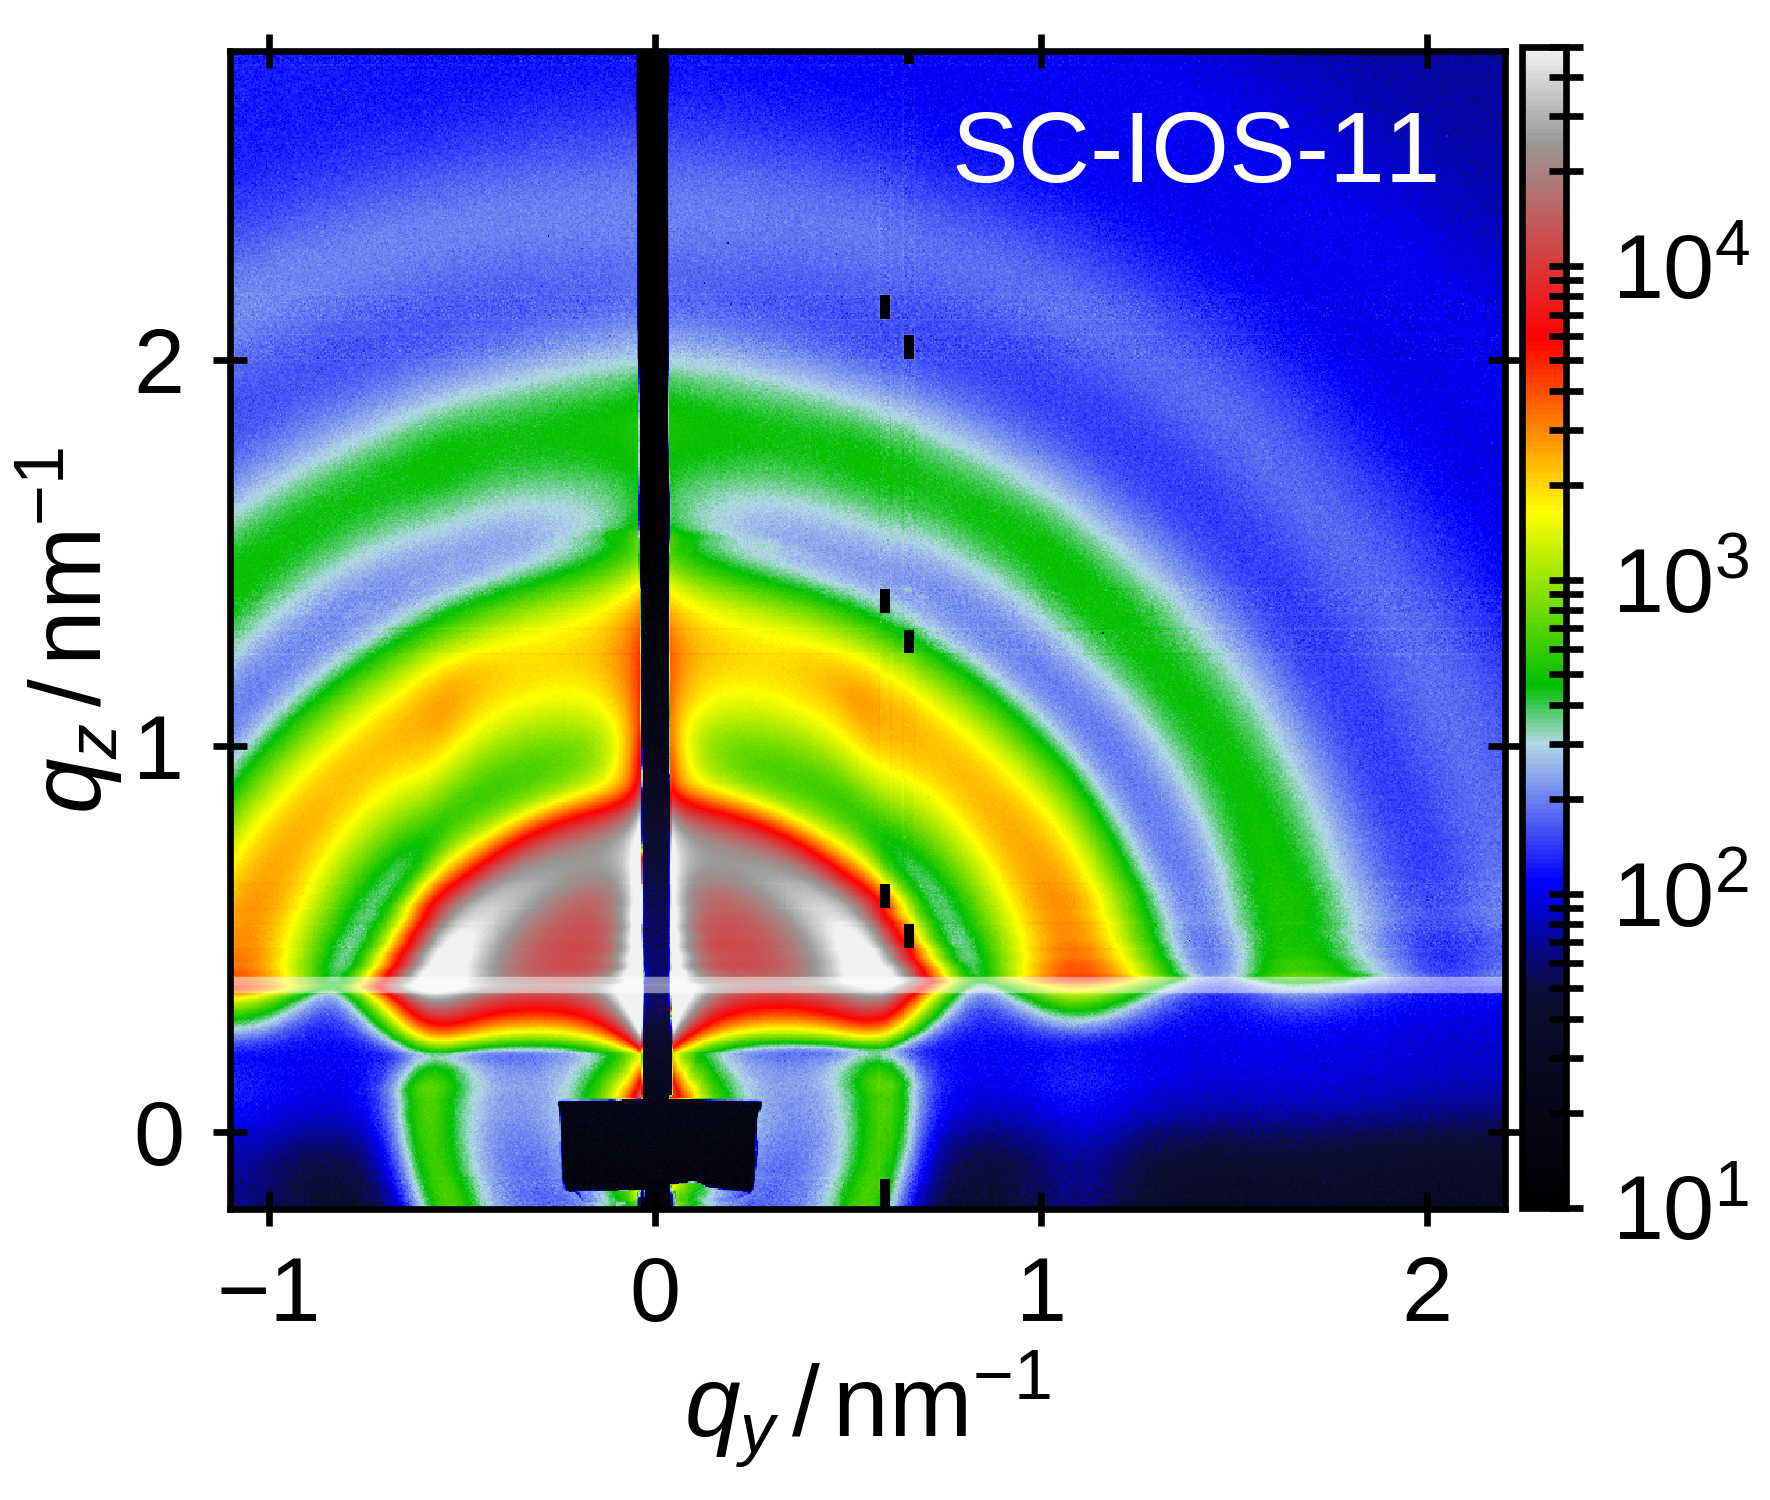
\includegraphics{looselyPackedNP_GISAXS_SC-IOS-11}
  %   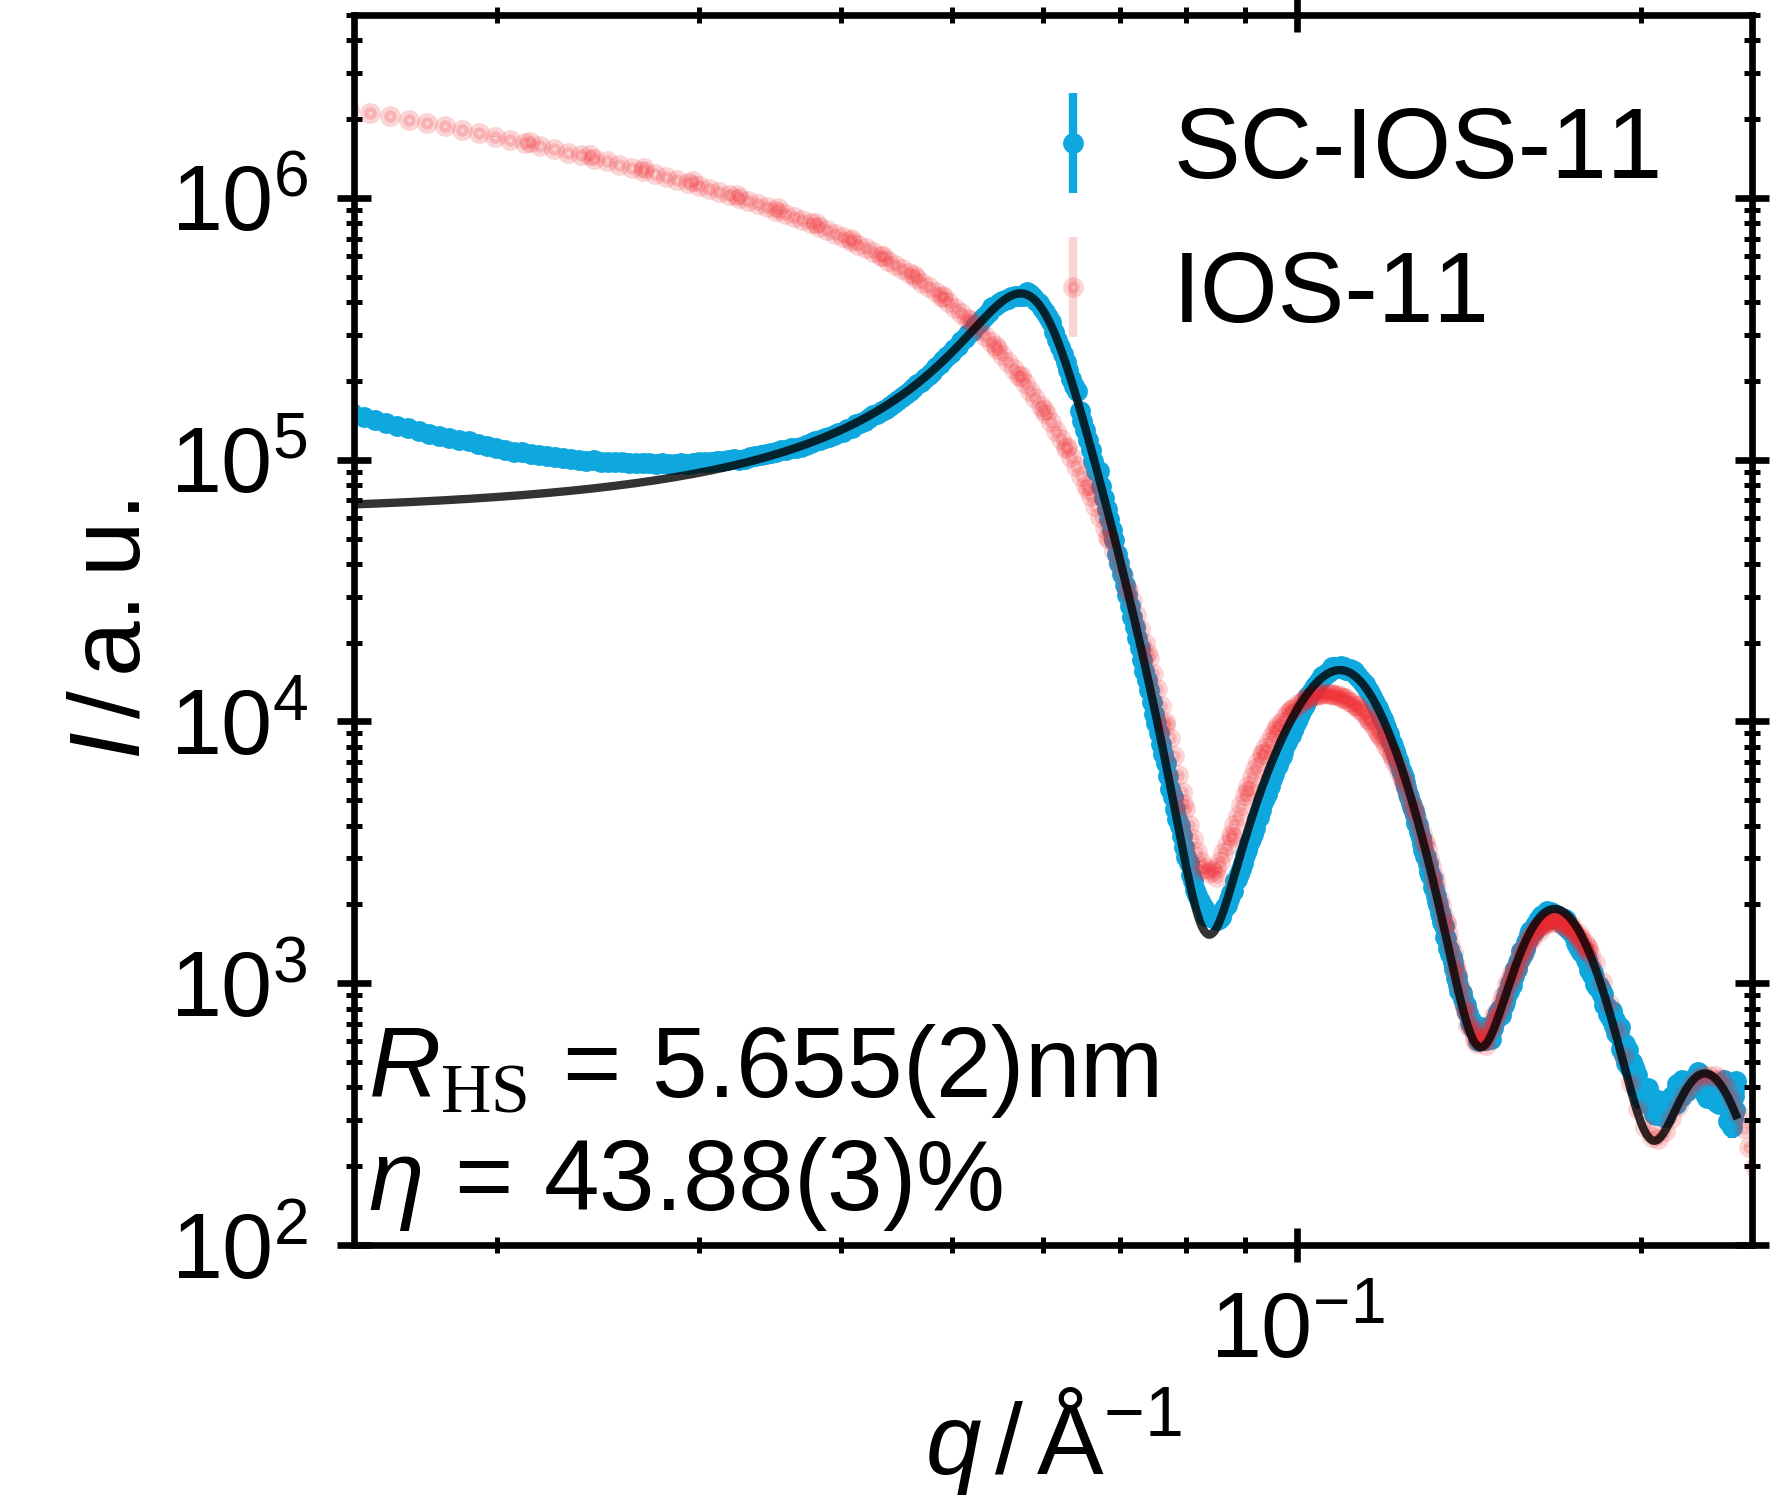
\includegraphics{looselyPackedNP_GISAXS_StructureFactor_SC-IOS-11}
  %   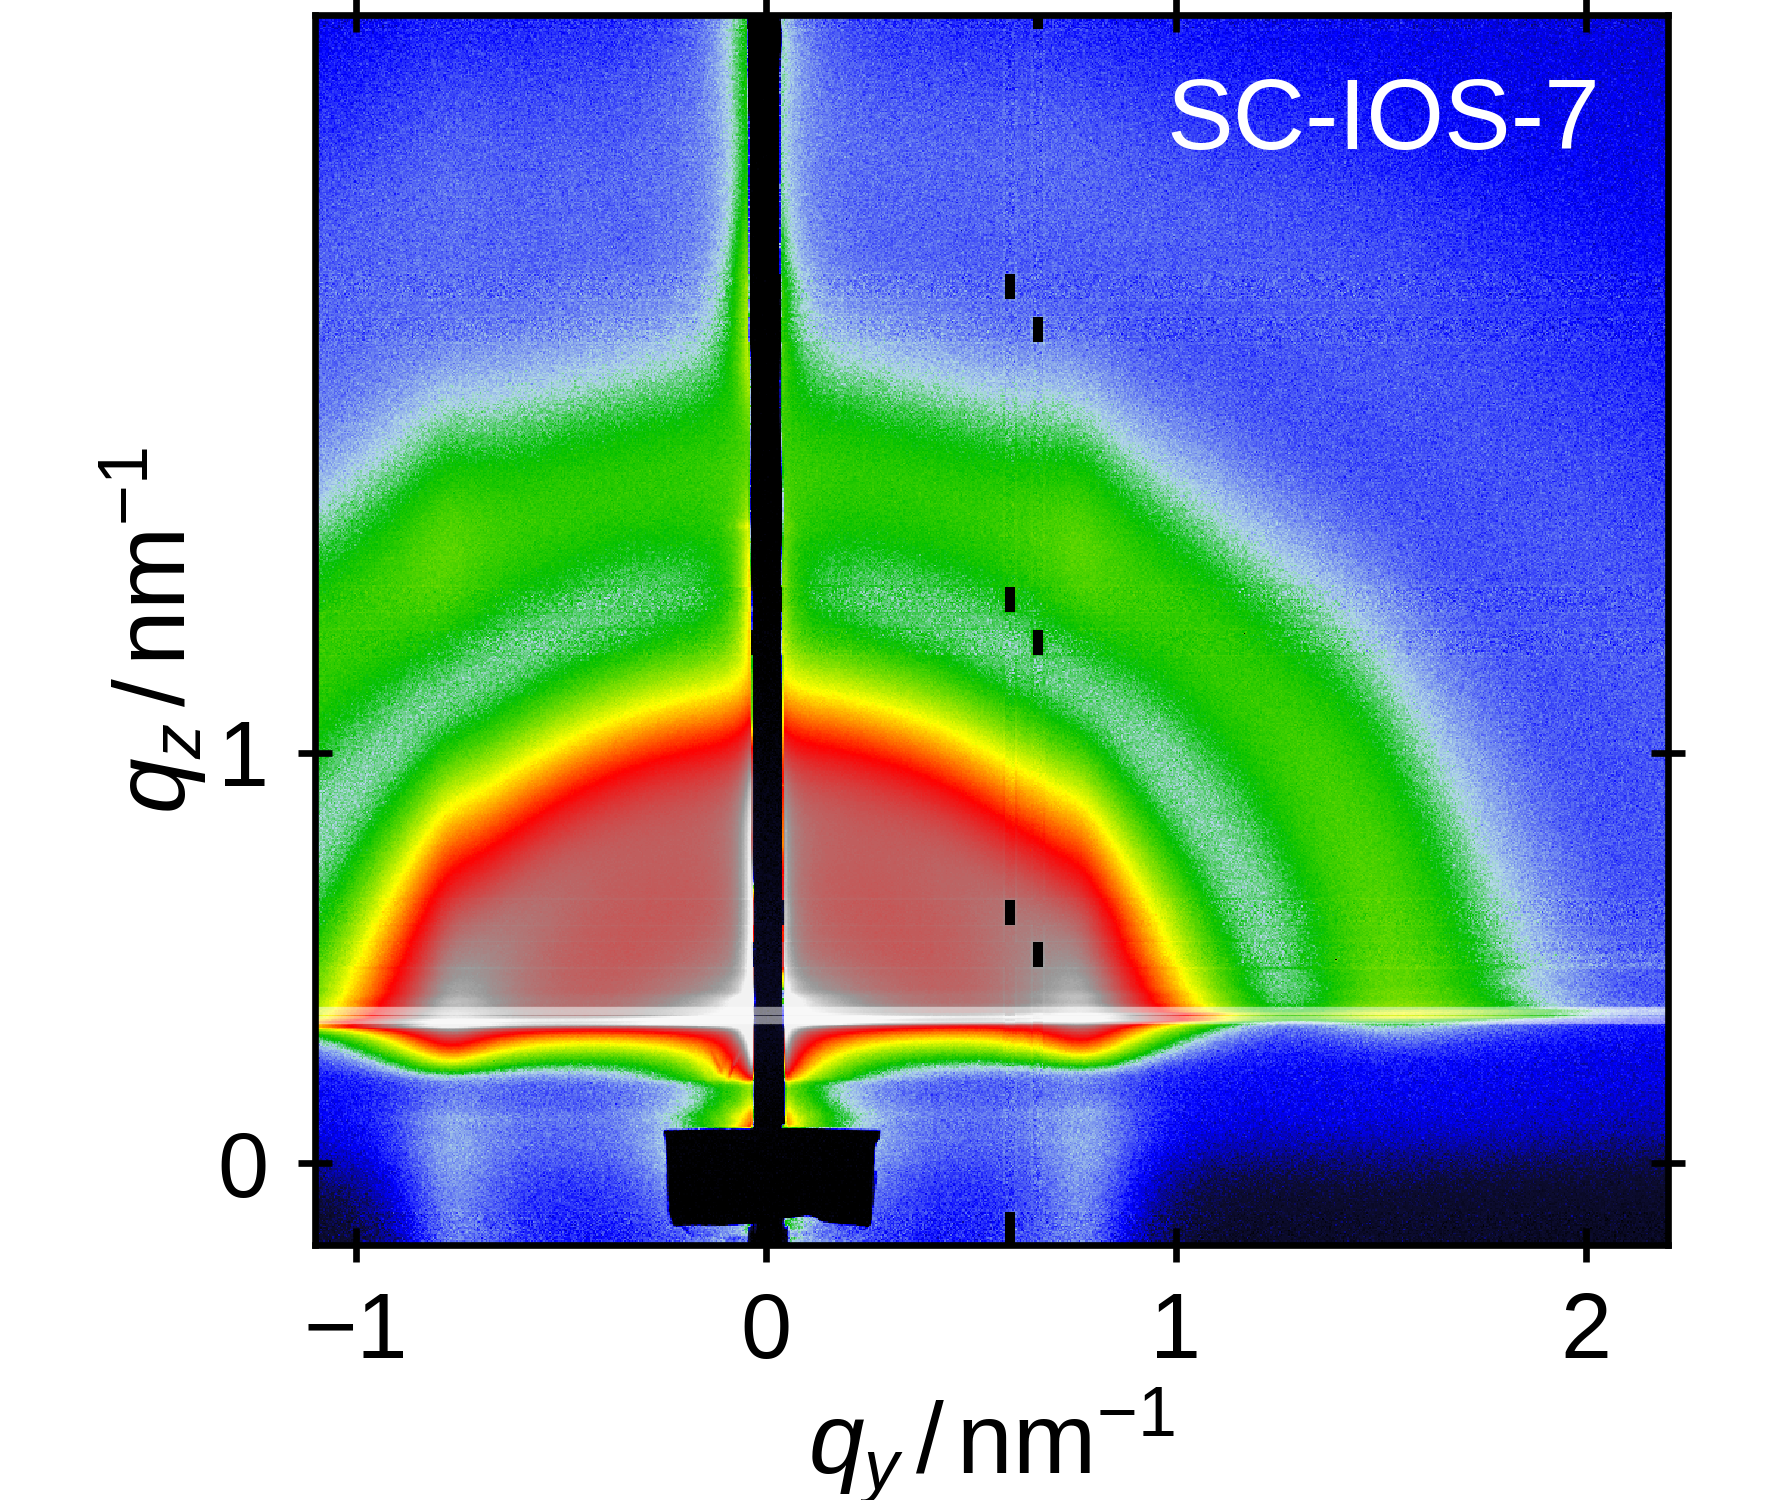
\includegraphics{looselyPackedNP_GISAXS_SC-IOS-7}
  %   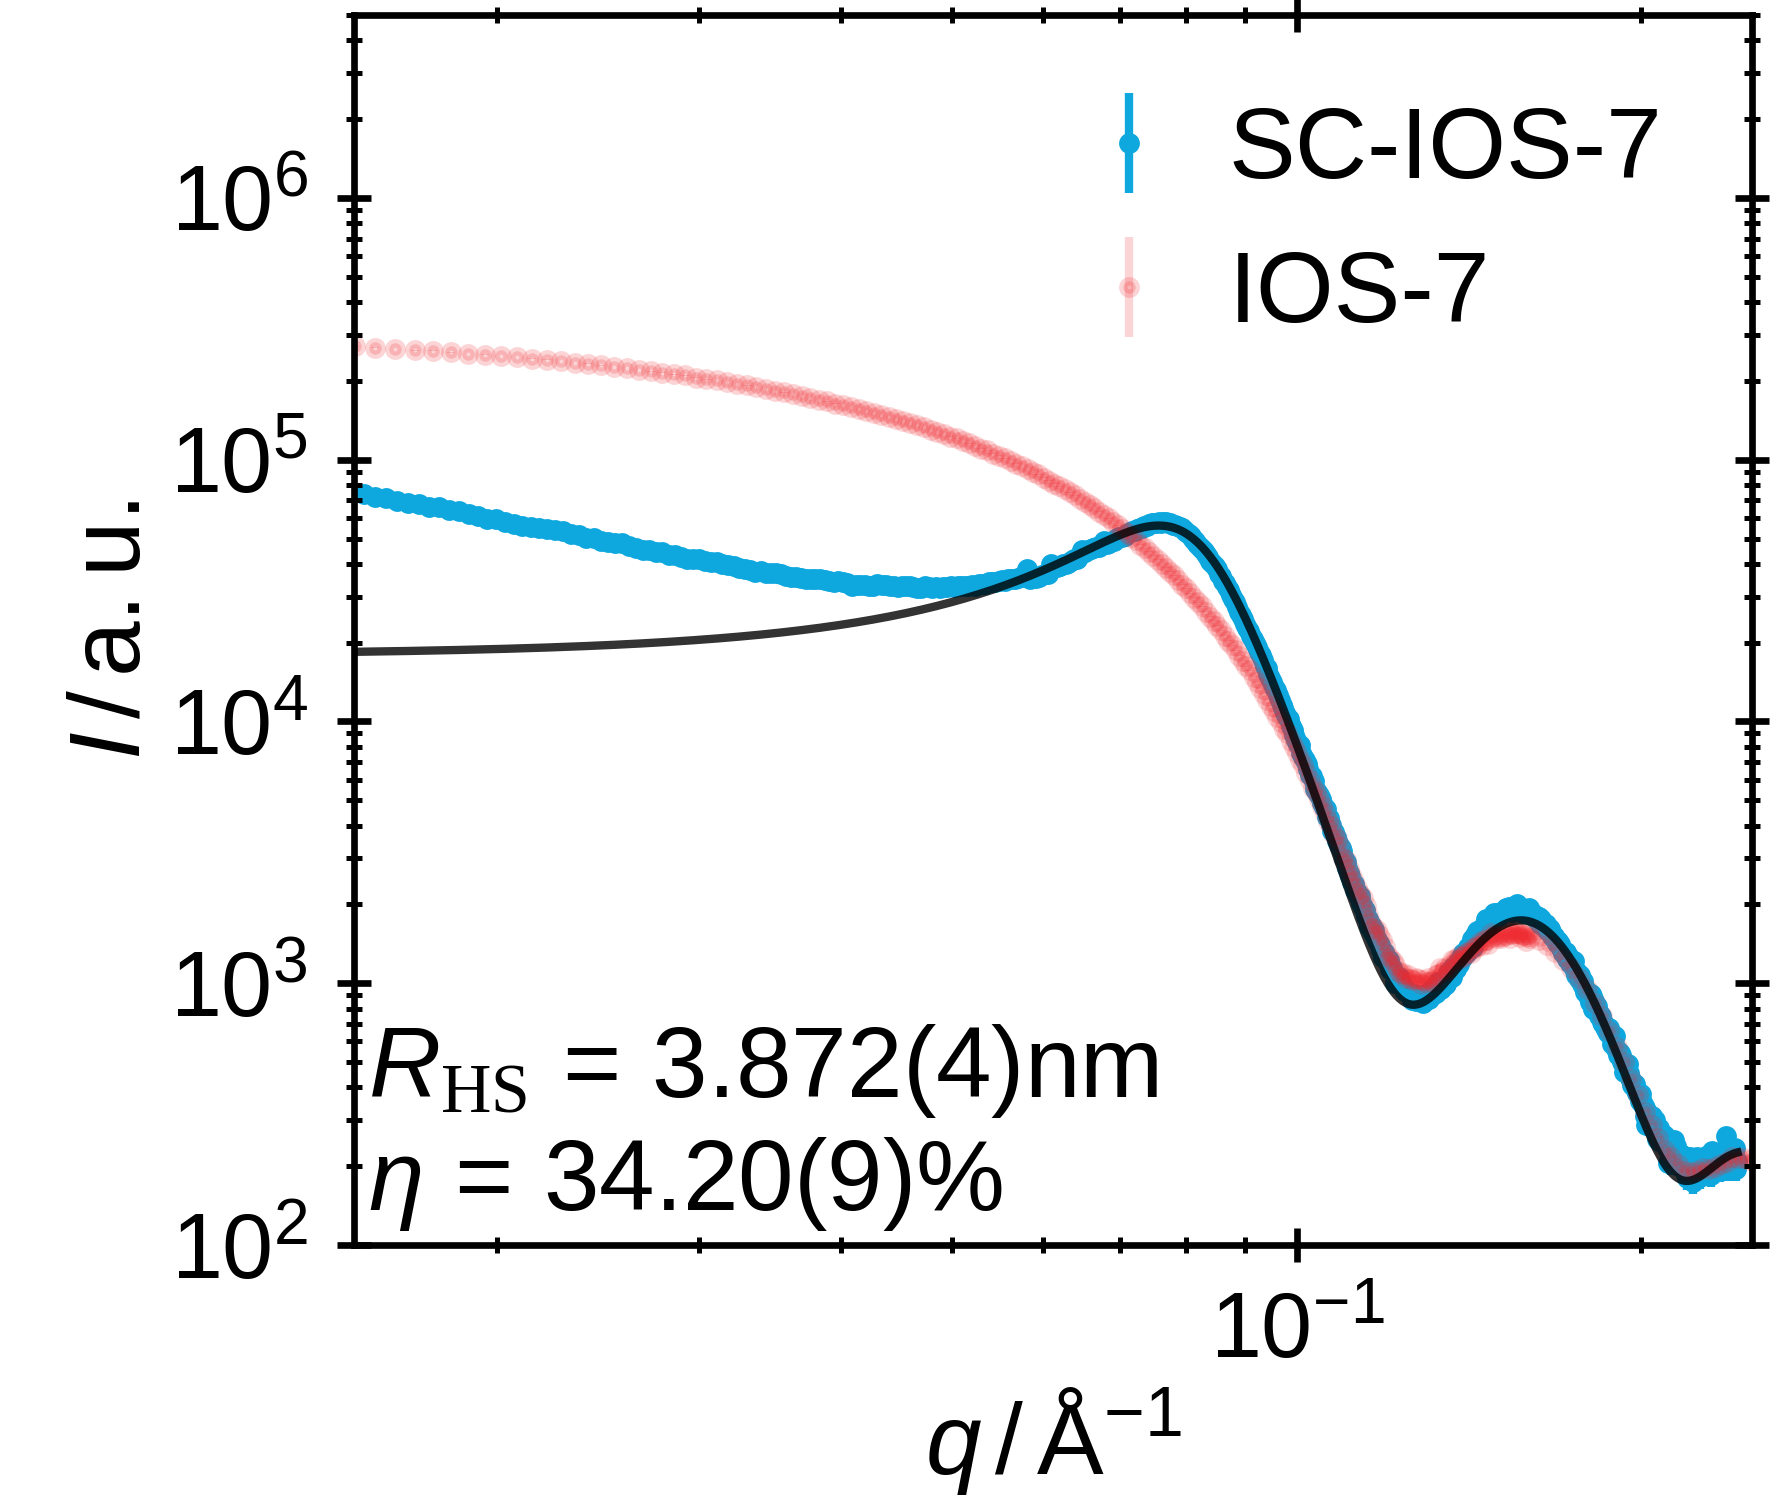
\includegraphics{looselyPackedNP_GISAXS_StructureFactor_SC-IOS-7.png}
  %   \caption{\label{fig:looselyPackedNP:layer:gisaxs}GISAXS detector images (left) of IOS-11 (upper) and IOS-7 (lower) measured at the BM26B beam line at the ESRF under an incident angle of $\alpha_i \eq 0.2 \unit{^\circ}$. The  integrated data in the Yoneda band (right, blue curve), marked by the white stripe on the detector images, is fitted to the hard-sphere structure factor in Percus-Yervick approximation, with parameters listed in \reftab{tab:looselyPackedNP:nanoparticle:gisaxs}. The SAXS form factor of the nanoparticles in dispersion is shown for comparison (red curve). The black area around $q_y \eq 0 \unit{nm^{-1}}$ is the beam stop, whereas the small black rectangles in the detector images are gaps due to inactive areas of the detector. }
  % \end{figure}

\end{document}